\chapter{国内外相关研究}
\label{chap:related_work}

本章主要介绍本课题的相关研究和实践工作,
其中包括现有的使用专业设备的高精度3D人脸重建方法,和基于少量非受限环境照片的3D人脸重建方法,
以及可微分渲染和它在人脸重建中的应用。

\section{使用专业设备的高精度3D人脸重建}

这类方法力求通过物理模型来精确描述被采集对象的形状和材质,从而在重新渲染时表现出很高的逼真度。
这些模型通常能从任意角度,在任意光照环境下重新渲染,以满足影视、游戏等领域的需要。

\begin{figure}
\centering
\begin{subfigure}[b]{0.53\textwidth}
    \centering
    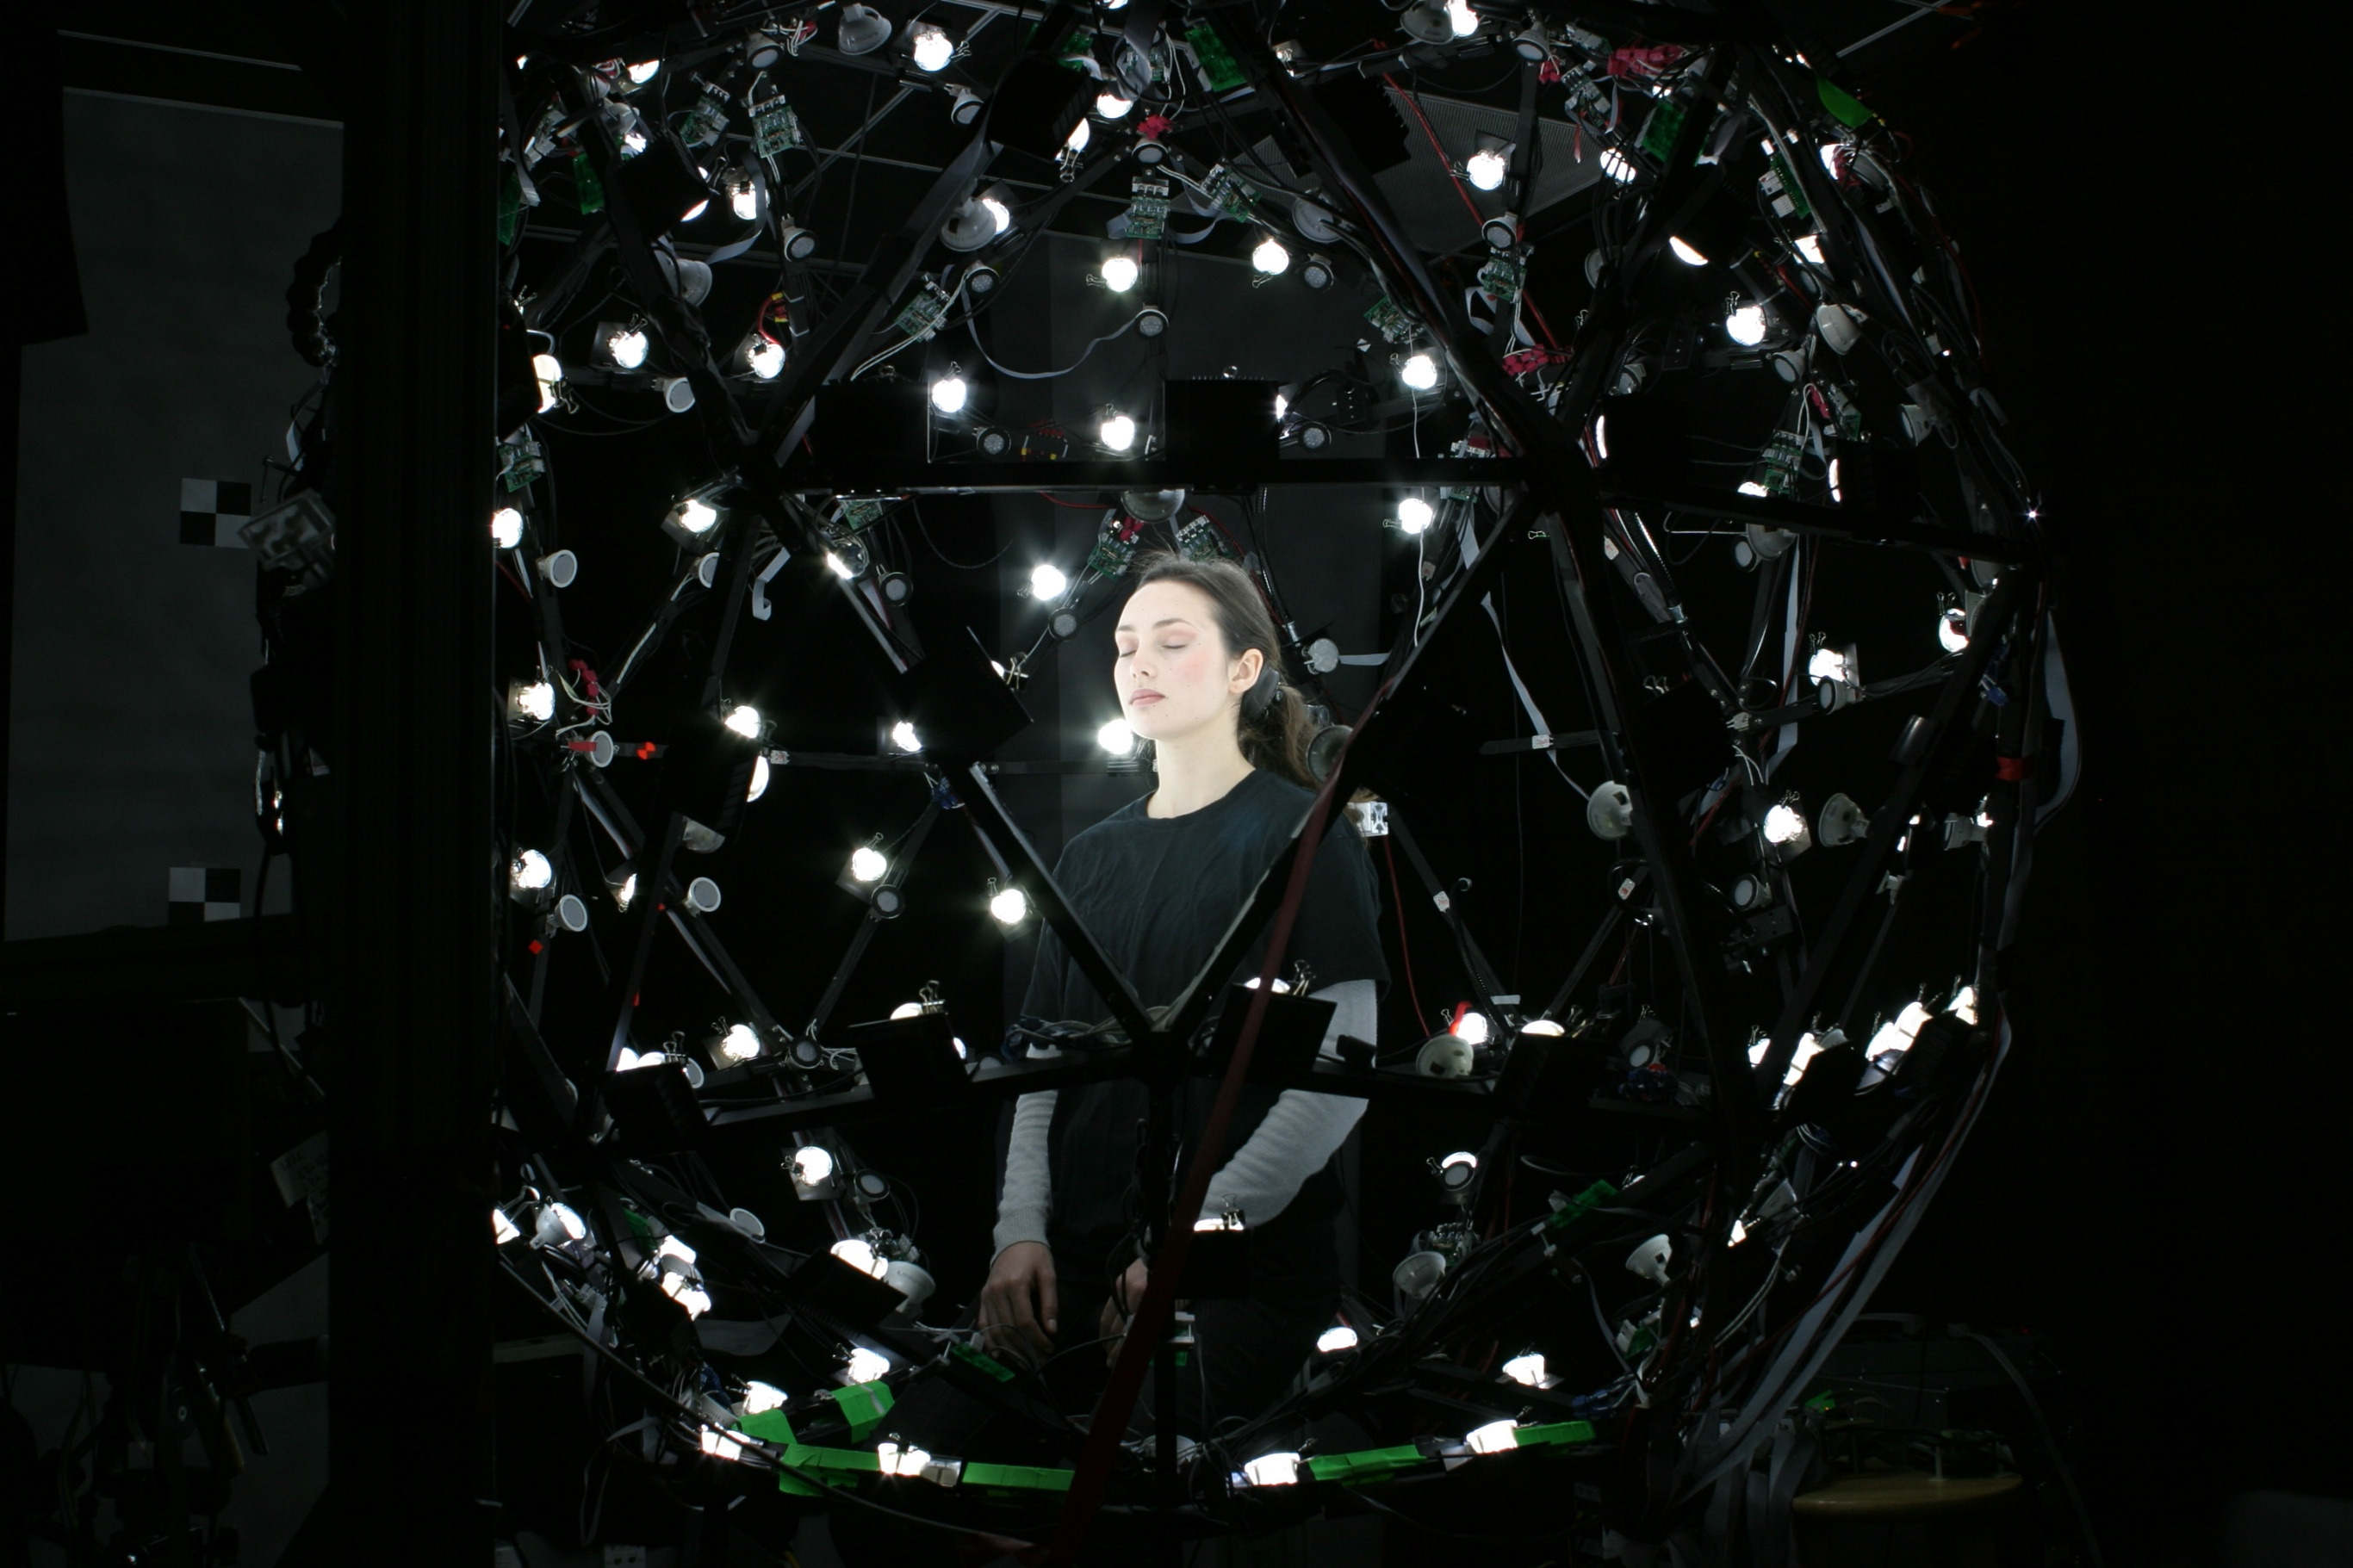
\includegraphics[height=160pt]{figures/light_stage}
    \caption{实际采集现场}
\end{subfigure}%
\begin{subfigure}[b]{0.47\textwidth}
    \centering
    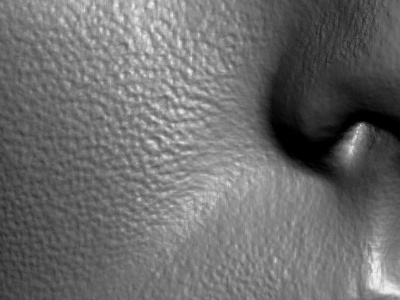
\includegraphics[height=160pt]{figures/emily_detail_1}
    \caption{重建的几何细节}
\end{subfigure}
\caption[Digital Emily 项目中的 Light Stage]{Digital Emily项目中的Light Stage\cite{DEP}}
\end{figure}

\paragraph{几何形状重建}
几何形状是物体最基本的属性,即物体每个部分在空间中所处的位置。
几何形状重建的基本方法是识别物体同一个部分在不同相机下的匹配关系,然后借助已知的相机参数,以及该部分在不同相机下的像素坐标,计算出该部分在3D空间中的坐标。
这类方法称为多目立体(multi-view stereo, MVS)。

而计算机中描述几何形状的方法有很多种,其中最基本的是点云模型,它保存了大量位于物体表面的点的坐标。
这种表示也是大多数几何重建算法的目标。
最初,\citet{PFM}通过在目标脸上画一些网格,从而允许手动建立格点间的匹配关系,并建立稀疏的点云。
\citet{ss_geo}对多个相机两两之间计算视差图,然后将多组视差图进行融合,并通过约束进一步排除误匹配点,最终得到一个稠密的点云。
其中视差图正是两张照片中,像素级别的匹配关系。视差图的构建是分辨率从低到高逐步细化的,并在过程中应用了平滑性、唯一性和顺序性的约束,以消除误匹配点。
\citet{DEP}则利用投影仪在目标表面投影彩条图案,以使匹配结果更加鲁棒。
3dMD的商业3D重建解决方案\footnote{\url{https://3dmd.com/}}也使用了斑点图案的投影。
D3DFACS\citep{D3DFACS}数据集采用了3dMD的方案。

虽然视差仍然是最广泛使用的方法,其准确度也非常高,但也不乏其他可行的方法。
例如,\citet{MaHPCWD07}使用光度立体的方法,通过多种球面梯度偏振光源的成像效果,重建物体的表面法向。高分辨率的法向信息可与中等分辨率的结构光的结果进行融合,从而获得高分辨率的几何形状,且能避免单纯依靠法线积分带来的累积误差。
\citet{phase_shift}则将相移方法与视差结合,以获得更高的准确度和鲁棒性。
\citet{BJUT3D}选择使用激光扫描仪。
FaceWarehouse\citep{FaceWarehouse}数据集采用了Kinect深度相机。

在得到点云之后,还需要将点云转换为网格,
该网格的拓扑结构应在采集的不同帧间,以及不同人物间保持一致,
以供渲染、人工编辑,动画制作等使用。
该任务的重点在于找到不同帧间的点的匹配关系,从而重建人脸的运动,变形等特征。
很多方法\citep{DEP,PFM,BickelBAMOPG07}通过在脸上画上易于识别的标记点以辅助匹配。但画标记点将给采集带来额外的工作量,且会影响到之后人脸材质的估计。
\citet{BeelerHBBBGSG11}通过图像空间跟踪和锚点帧的方法,获取稠密且累积误差小的匹配关系,从而将网格的拓扑结构传播到所有帧,再逐帧根据点云进行微调。
FLAME\citep{FLAME}则完全依靠3D数据,而不使用照片。FLAME是一个由少量PCA得出的参数控制的3D网格模型。它交替地训练该模型和将该配准到3D数据上,从而找到3D数据间的匹配关系。
但3D数据中所包含的信息量有限,因此完全依靠3D的数据的理论精度应不如跟踪图像的方法。
也有一些方法能直接从照片中重建网格,而不需要先得到点云。
\citet{LiLBL0Z21}以传统方法的结果为训练数据,训练一个神经网络,通过体素特征,由粗到细地直接生成网格。

近年来,随着神经辐射场(NeRF)\citep{nerf}等技术的发展,也有一些方法将几何形状编码在神经网络等隐式表达中,而不使用点云、网格等显式表达。
NeRF\citep{nerf}首先提出将几何信息编码在用神经网络表示的密度场中,然后通过体渲染的方法,将渲染结果直接与照片比较,从而优化该模型。
然而,这类隐式模型虽然构建简单,但有诸多问题,例如难以进一步人工编辑,渲染效率较低等。
MoRF\citep{MoRF}通过神经网络生成的形变场以表示人脸几何形状,从而将几何形状和材质分离,提升了可编辑的程度。
\citet{nvdiffrec,nvdiffrecmc}先优化在可变形四面体网格中存储的有向距离场,然后将其转换为传统的显式三角形网格,并使用可微分渲染进一步优化。以此解决隐式模型不易编辑的问题。

\paragraph{相机标定}
精确的相机标定是精确的多视角3D重建的基础。
目前主流的标定方法是用相机拍摄特制的标定目标。
\citet{ss_geo}采用在一个球形目标物体上随机地粘贴一些可识别的角点。
其优势在于不同角度下都能观察到较多角度较正的角点。
\citet{del_grid}提出使用三角形网格代替正方形网格,以在角点处提供更多的梯度信息,从而提升角点定位的精度。
\citet{SchopsLPS20}提出使用大量参数来描述相机模型,且大幅提升标定目标中角点的数量和角点中的梯度信息,从而更精确地估计这些参数。

\paragraph{材质估计}
材质指的是物体的表面法向、颜色、粗糙度、金属度、次表面散射等属性。
更宽泛地说,材质描述了物体将如何与光线相互作用,即如何吸收,折射,反射,散射入射的光线。
若要获得高质量的,可在任意光照条件下渲染的3D模型,则必须对材质进行建模并估计模型参数。

在采集时直接收集多种不同光照条件下的照片的方法称为\emph{主动光源方法}。
第一代Light Stage\citep{light_stage}使用一个可绕人脸自动旋转的光源,从而获得人脸对各个方向入射光的响应情况,从而实现任意光照条件下的渲染。
此外,该作者还利用色彩空间分析技术\cite{temporal_color}对脸部的法线分布,颜色等属性进行建模,从而实现了任意视角下的渲染。该方法的缺陷在于其单帧图像的采集时间较长。
\citet{MaHPCWD07}通过LED阵列实现的偏振球面梯度照明将所需采集的照片数量减少到了8张,耗时也大幅减少。该方法也通过混合法向模型获得了较为真实的渲染效果,尽管在原理上不太符合物理模型。
此后\citet{KampourisZG18}进一步提出使用球面二值照明和色彩空间分析\cite{MallickZKB05}以分离镜面反射。同时该方法进一步减少了所需采集的照片数量。
\citet{FyffeGTGD16}的方案与本文的方案更为类似。该方法使用了6盏闪光灯并依次在几十毫秒内触发,并用24台相机分布在不同闪光灯闪光时触发快门。该方法可以在近乎瞬间完成6种不同光照的采集,从而避免了被采集对象可能的运动。
\citet{ZhangZZLCYXY22}使用了高达1000FPS的相机,搭配精密控制的LED阵列,实现了在通常一帧的时间内完成数十种不同光照条件的采集。
以上方法使用时域复用的方法来收集多种不同光照条件下的数据,但也有一些方法\citep{FyffeD15,MekaHPZFFKYBDDB19}采用频域复用的方法,即使用可以分别控制不同波长的光的强度的RGB LED灯,在不同频率下实现不同的光照条件。

与之相对的是\emph{被动光源方法},即在采集时光照条件保持不变。这类方法的硬件实现通常更为简单。但缺失的信息则需要通过多视角或者更强的正则化等来弥补。
在早期,直接使用照片中的颜色作为漫反射反射率的估计值的方法\citep{PighinHLSS98,BradleyHPS10}比较常见。但这种做法在光源和视角变化时逼真度太低。
\citet{GotardoRBGB18}使用了一个一维子空间来建模人脸在形变过程中反射率的变化,从而大幅限制解空间的维度。但该方法需要在开始阶段让目标缓慢转头采集多帧以初始化该子空间。所以该方法相当于将主动和被动光源相结合。
\citet{RiviereGBGB20}使用了带有次表面散射的材质模型,分别采集了不同偏振方向的数据以更好地分离镜面反射和次表面散射。该方法实现了纹理空间的可微分渲染以估计模型中的参数。
在此基础上,\citet{XuRZCBG22}使用了更准确的偏振模型,光源模型,并建模了部分间接照明效果,使估计的材质参数更加准确。
\citet{nvdiffrec}使用通用的粗糙度-金属度材质模型,利用可微分光栅化渲染技术,联合优化模型的几何形状和材质参数。由于联合优化的难度较高,该方法需要大量的视角作为输入。
本文中的实验平台将会同时支持主动和被动光源方法,以详细探究不同光照条件对重建效果的影响。

除了这些直接描述物理性质的参数化材质模型外,也有研究希望能使用神经网络作为材质模型。
例如NeRF\citep{nerf}也可建模并输出物体反射光线的颜色和强度,且可以建模反射随视角变化的变化,但无法建模与采集时不同的光照条件下的反射情况。
MoRF\citep{MoRF}则通过输出传统着色所需的材质参数,而不是直接输出反射光线,从而能够适应任意新的光照环境。

总结来说,以上这些方法通常使用较为通用,参数量较多的模型,并通过采集尽可能多的数据,通过物理原理来准确估计模型参数,以期尽可能准确的还原采集目标在现实中的样子。

\section{基于非受限环境照片的3D人脸重建}

上述这些方法虽然能逼真地重建人脸模型,但都需要专用的设备和环境来采集数据,这大大限制了他们的应用场景。
除上述这些成本不敏感而力求准确的方法外,还有一些方法则希望降低采集的设备成本和复杂度,从而推动3D人脸重建技术在更多领域的应用。
这些方法通常建立在上述高精度方法的基础上,通过采集大量人脸的数据,从中学习并建立更多的关于人脸的先验知识,从而大大降低解空间的维度。
得益于此,它们甚至可以实现从单张非受限环境中拍摄的照片中重建3D人脸\citep{danzhangtuxiangsanwei}。
但相对应地,受限于先验知识,这些方法重建的结果可能缺失高频信息,或者产生逼真但不准确的结果。

\subsection{3D人脸统计模型}

引入3D人脸统计模型是向重建算法中添加这些先验信息最常用的方法,
因为它们在对大量3D模型的统计过程中,在模型参数里编码了不同人人脸的几何和外观变化。
这些模型通常可以从一个低维的特征向量中生成一个较复杂的3D人脸模型。
于是,3D人脸重建的过程可以被看做估计一个特征向量,以及相机姿态和环境光照,使得其对应的模型渲染后与输入的照片尽可能地相似。
这大大降低了解空间的维度。

其中使用范围最广的3D人脸统计模型是3D可形变模型(3D morphable model, 3DMM),
它最初是由\citet{3DMM}提出的。
一个3DMM通常包含独立的几何形状模型和反射率(又称颜色,纹理)模型。
这两者是分别通过PCA得到的。
为构建一个3DMM,首先需要采集大量的3D人脸模型,并将每个模型表示为一个包含3D网格顶点坐标的形状向量,以及一个包含每个顶点颜色的反射率向量。
3DMM背后的思想是:如果采集的3D人脸模型足够多,那么任意一个3D人脸模型都可以通过对这形状和反射率向量的线性组合来表示。
于是任意新的人脸可表示为该线性组合的权重。
但当采集的数据集中的人脸数量较多时,这些权重的维度也会较高。
PCA可以用于降低维度,并去除冗余的数据。
若对数据集中的形状和反射率向量分别进行PCA,可分别得到形状和反射率的均值、特征向量和对应的特征值。
部分特征值很小的分量可被忽略,
剩余的部分即是在下游的3D人脸重建过程中所需要的3DMM模型。
与大量人脸数据相比,通过对少量特征向量的线性组合,即可覆盖原数据集中线性组合权重空间的大部分区域。

虽然3DMM仍是使用最为广泛的3D人脸统计模型,但它也有一些局限性。
首先,PCA产生的特征向量建模了数据集中变化的主要方向,所以一些微妙的细节,如皱纹等,并不能被捕获,
因此难以通过拟合3DMM的方式重建人脸细节。
对此,\citet{ferrari2017dictionary}提出了一种基于矩阵分解的方法,将数据集中的形状向量构成的矩阵分解,从而获得稀疏性。
\citet{brunton2014multilinear}对数据集中的样本应用小波变换,从而获得人脸表面的多尺度分解,然后对小波系数构建局部多线性模型。
\citet{jin2017robust}使用非负矩阵分解(NMF)以将形状分解为局部特征。
最后,\citet{luthi2017gaussian}将形状的变化建模为高斯过程,并在全局的模型上添加了局部模型,从而结合了多尺度的信息。

另一点局限性是,3DMM所假设的线性组合的模型表现力不够,可能并不足以精确建模新的人脸。
于是有另一些方法通过3D模型的自动编码器来学习一个人脸形变的隐空间。
FLAME\citep{FLAME}在模型中加入了骨骼绑定来建模下巴和转头等较大的形变,
\citet{jiang2019disentangled}则估计了两个独立的隐空间,一个用于编码身份相关的形变,另一个用于编码表情相关的形变。
在自动编码器的结构上,\citet{ranjan2018generating}和\citet{jiang2019disentangled}使用了频谱卷积操作,
\citet{bouritsas2019neural}则使用了带有各向异性卷积核的螺旋卷积操作,这使得顶点的邻居可以和卷积核参数一一对应。
这类方法均试图使用神经网络来代替3DMM中的线性组合,从而提高模型的表现力。

\subsection{统计模型拟合方法}

在有了统计模型中编码的人脸先验知识之后,
3D人脸重建的过程就可以被看做是优化统计模型的参数,使其输出的图像与输入的照片尽可能地匹配。
本文后续章节所使用的方法也属于这一类方法。

与利用多视角图片相比,从单张非受限环境的照片中重建3D人脸具有更广泛的应用,但也更难,因此大多数研究主要关注基于单张照片的重建。
但也有一些方法\citep{deep3d,piotraschke2016automated}利用同一个人在不同环境和姿态下的多张照片以提高重建的准确性。
另一些方法\citep{ShiWTC14,GarridoVWT13}则提出使用视频作为获取同一个人的多张图片的简单方法。

\paragraph{优化非线性损失函数}
\citet{3DMM}不仅首先提出了3DMM模型,而且也介绍了一种将该模型拟合到单张人脸照片的方法,并启发了大量后续的研究。
该作者使用了逆渲染的思想:如果重建的模型渲染的效果与输入的照片相似,那么认为这个模型忠实地重建了输入的照片中的人脸。
作者使用可微分渲染的方法,将渲染图像与照片进行匹配,以梯度下降的方式优化3DMM的形状和反射率参数、以及相机和光照等渲染参数。
该方法仍需要人工指定一个较为准确的初始化。
在其后续工作\citep{BlanzV03}中,作者引入了在照片中手工标注的人脸关键点作为额外监督信号。
利用类似的方法,\citet{piotraschke2016automated}将同一个人的多张照片的重建结果组合起来,以获得单个更准确的模型;
\citet{cai2020}利用了多视角图像,并通过光流和明暗关系恢复人脸细节;
\citet{thies2016face2face}根据重建的模型,将表情在不同照片间迁移。
一些方法提出了对关键点损失的改进。
\citet{qu122015adaptive}将关键点分为内部和边缘两类,为解决边缘关键点在侧脸照片中定义不明确的问题,作者提出了一种自适应的边缘关键点选择方法。
\citet{liu2019single}在估计人脸形状和相机参数的同时,迭代地更新边缘关键点的位置,以改善3D模型和照片中关键点的对应关系。
\citet{zhu2015high}则是联合估计边缘关键点的位置和其他参数。
这些方法试图以边缘关键点的方式使模型对齐到照片边缘。
然而,关键点的监督是稀疏的,可能造成不准确的结果,且这些方法在关键点识别的基础上又增加了额外的复杂度。
本文后续章节将介绍一种直接利用可微分渲染中的可见性梯度实现对齐的方法。

除了上述提到的关键点和直接的像素损失外,还有一些方法使用了其他损失函数。
\citet{sariyanidi2020inequality}计算了图像间梯度的关联性,并且用不等式约束代替了通常使用的正则化项。
\citet{booth20183d}使用了一个特征纹理代替了原3DMM中的反射率模型,并在渲染后,与从照片中提取的特征计算损失函数。
\citet{gecer2019ganfit}则直接使用人脸识别神经网络提取的特征来计算损失函数。

\paragraph{概率方法}
\citet{schonborn2013monte}提出了一种非常不一样的拟合3DMM的方法,
他们将该问题重新定义为一个概率推理问题,即给定一个人脸照片,他们从后验分布中不断采样新的参数,并概率性地接受或者拒绝这些新的样本。
其后续工作\citep{SchonbornEFV15}与本文第\ref{chap:method}章中希望解决的问题类似:希望逆渲染任务能更加适应未知背景的环境。
但该作者的思路是对背景应用一个较为通用的模型,且采用的是非基于梯度的离散优化方法。
本文将在现有计算可见性梯度的方法的基础上,提出一种无需为背景建模的,适应未知背景的梯度计算方法。

\subsection{深度学习方法}

上述方法中使用到的先验信息大多仅编码于人脸统计模型中,
而本节所述深度学习方法则直接学习从照片到3D人脸模型的映射,将先验信息编码于神经网络的参数中。
这类方法鲁棒性好,且由于推理时不需要迭代优化,其效率一般可以达到实时。
然而,他们遇到的主要问题是缺乏足够的3D人脸扫描作为训练数据,后续研究者们也通过各种手段缓解了该问题。

其中一个使用较为广泛的方法是使用合成的数据集进行训练。
\citet{zhu2016face}首先用3DMM拟合真实人脸照片,然后将3D模型旋转并重新投影回图像上,以此生成和原始照片相似但人脸角度更大的照片。
该作者使用该技术创建了300W-LP数据集,并被之后很多工作所使用。
与该策略相似,其他很多方法\citep{trần2018extreme,chaudhuri2019joint}直接使用了3DMM拟合的结果作为神经网络的监督信号。
此外,还有很多方法采用了完全生成的数据集,
它们大多从3DMM中随机采样参数,然后使用随机的光照和相机视角渲染得到图像。
这类方法的优势在于,其图像和3D模型间的对应关系是绝对准确的,且不依赖于3DMM的拟合质量。
但渲染的图像往往不够真实,这样的模型在现实照片上的表现可能不佳。
\citet{richardson20163d}使用了Phong反射模型合成图像。
\citet{dou2017end}则在使用合成数据的同时也使用了真实的扫描数据,以提升其在真实照片中的表现。
\citet{genova2018unsupervised}则使用两阶段的训练方式,先使用合成数据监督训练,再使用无标签的图像无监督地训练。

一些更新的方法则完全摆脱了对3D数据的依赖,它们可以直接从无标签的人脸照片中学习。
这些方法在神经网络输出的3D模型后面增加了一层可微分渲染层,并直接优化渲染图像和输入照片间的误差。
这类方法可以看作深度学习与前述优化方法的结合。
\citet{deep3d,bao2022}利用已有的人脸关键点识别算法和可微分渲染来直接从大量人脸照片中学习预测3DMM参数。
DECA\citep{DECA}则在重建FLAME模型的基础上,额外添加了表情相关的动态细节。
\citet{ZielonkaBT22}利用人脸识别算法提取的特征,试图降低人脸远近和大小间的歧义,重建物理尺度更准确的3D人脸模型。
此外,该作者也使用了可微分渲染来捕获输入中的表情,弥补人脸识别对表情的不敏感。
\citet{shen2022,feng2018prn}则选择了不输出3DMM模型的参数,而是直接输出3D人脸模型的顶点坐标。
还有很多方法\citep{CaoBZB15,IchimBP15}也是使用类似的思路从单目照片或视频中重建3D人脸,并通过图像中的线索为3DMM模型添加更多细节,使其更加逼真。

以上方法的输入均是在非受限环境下拍摄的照片,其环境光照信息是未知的。
但在实验室的受控环境下,也有一些方法通过数据建立更多的先验知识从而减少所需采集的数据量。
\citet{MekaHPZFFKYBDDB19}通过图片到图片的神经网络,输入两张RGB梯度照明的照片,生成稠密的反射场,从而实现了任意光照条件下的渲染。但该方法作为2D方法,无法简单地扩展到任意视角的3D渲染。且神经网络的输出虽然看上去非常逼真,但在物理上可能不够准确。
\citet{ZhangZZLCYXY22}使用多个VAE分别对采集到的人脸的表情、几何形状、纹理进行解耦、编码和生成,从而实现高效地编辑、驱动所捕获的高精度人脸模型。

\section{可微分渲染}

可微分渲染旨在求解渲染得到的图像关于渲染参数的梯度,以解决逆渲染问题,即从渲染结果的图像中恢复渲染该图像所需的参数。
前述的很多3D人脸重建方法都使用到了可微分渲染相关的技术作为其合成分析方法的一部分,但其运用还很初级。
例如,现有方法均只对每个像素的着色过程计算了梯度,而忽略了几何遮挡等因素。
本文也试图推进更现代的可微分渲染在3D人脸重建中的应用。
下文将介绍通用的可微分渲染领域的一些研究。

\paragraph{基于光线追踪的可微分渲染}
这类方法通过光线追踪的方法,通过蒙特卡洛采样,模拟大量光线在场景中的传播,无偏地估计每个像素的颜色,同时计算该过程的梯度。
这类方法通常计算量较大,且由于随机采样,其估计的梯度具有一定噪声。
\citet{redner}提出了一种使用蒙特卡洛光线追踪的可微分的基于物理的渲染方法,其具有正确的可见性梯度。
Mitsuba 2\citep{Mitsuba2}是一个多功能的渲染框架,可以用于解决各种渲染问题。
它创新性地使用了一种重参数化技术来计算几何遮挡相关的梯度。
\citet{ZeltnerSGJ21}提出将渲染过程和求微分过程的采样解耦,从而降低梯度估计的噪声。

\paragraph{基于光栅化的可微分渲染}
第二类可微分渲染方法旨在提高性能,以支持合成分析中迭代优化所需的大量迭代次数。
这类方法基于实时渲染中使用的光栅化渲染方式。
它们使用局部信息渲染和着色3D网格,而忽略遮挡和反射等全局光照现象。
这类方法的难点依然是如何计算几何遮挡相关的可见性梯度。
\citet{softras}将每个三角形光栅化为具有可配置模糊半径的概率云,这些云根据其他可配置参数进行启发式组合。这种模糊使覆盖率成为关于顶点位置的连续函数,这对于获得可见性梯度是必要的。
但是,模糊也意味着不透明表面在边缘周围变得透明,从而导致图像不正确。因此需要人工调整这些参数以在图像正确性和梯度质量之间达到平衡。
DIB-R\citep{ChenLGSLJF19}输出一个额外的alpha通道,该通道通过可配置的模糊半径扩展到覆盖像素之外。该alpha通道可用于近似可见性梯度,但仅当参考图像也有alpha遮罩时才能使用。
此外,位于其他几何体前面的轮廓也无法获得可见性梯度。
其模糊半径的参数也需要人工调整。
\citet{KatoUH18}在反向传播过程中基于几何信息在三角形边缘上近似出基于图像的梯度。但是,这些梯度与渲染的图像不一致。
\citet{nvdiffrast}提出了一个模块化的渲染器,其中抗锯齿模块可产生可见性梯度,但它需要处于边缘的三角形正好被渲染到了图像中,否则其产生的梯度就较为稀疏,给优化带来偏差。
\citet{ColeGSVZ21}提出了一种在离散的光栅化算法的基础上解算可见性梯度的方法。该方法也会引入少量模糊。
\citet{LyuHL0TT21}使用球作为代理,为渲染加上了近似的阴影。以更好地拟合目标图像。

这些研究大多均试图解决可见性梯度的计算问题,
但他们都是针对整张图片计算的,并未考虑到照片中可能存在的难以建模的背景。
本文将在这些方法的基础上,提出并实现了一种在未知背景的情况下利用可见性梯度的方法。

\section{基于物理的高质量人脸3D渲染}

若要通过逆渲染的方法,基于可微分渲染重建3D人脸,首先需要一个高质量的3D人脸材质模型和渲染器。
本节将简要介绍计算机图形学业内常用的人脸3D渲染技术。

\paragraph{基于物理的渲染}

在早期的实时3D渲染中,由于计算性能的限制,模型的着色通常是基于一些简单的经验公式的。
而如今,基于物理的渲染(PBR)已经成为了主流,其渲染效果更加逼近真实世界的光照效果。
在基于物理的渲染中,材质模型通常表征了材质的一些物理属性,使其可以直接从现实中测量得到。其渲染方式也是对物理过程更加真实的近似。
这也给从照片进行逆渲染奠定了基础。

其中当前应用较为广泛的模型之一是迪士尼提出的Disney BSDF模型\citep{PBR_disney}。该模型可广泛用于描述生活中的绝大多数材质,包括金属、塑料、玻璃、橡胶、布等。
该模型由迪士尼应用于自己电影的离线渲染中,后被Blender、Unreal Engine等渲染器借鉴。
该模型的参数包括:
基础颜色,表征了材质对不同波长的光的反射率;
金属度,表征了材质是金属或电介质;
粗糙度,表征了材质表面的粗糙程度;
镜面反射,取决于物体的折射率;
以及其他一些共十余个参数。
这些参数也即在3D重建中所需求解的参数。

\paragraph{次表面散射}
除了上述参数外,次表面散射效果在人脸上较为明显,且其渲染较为复杂,因此在此单独介绍。次表面散射是指光线在入射物体之后,在其表面附近多次散射,再从与入射不同的位置出射的现象。

\begin{figure}[bth]
    \centering
    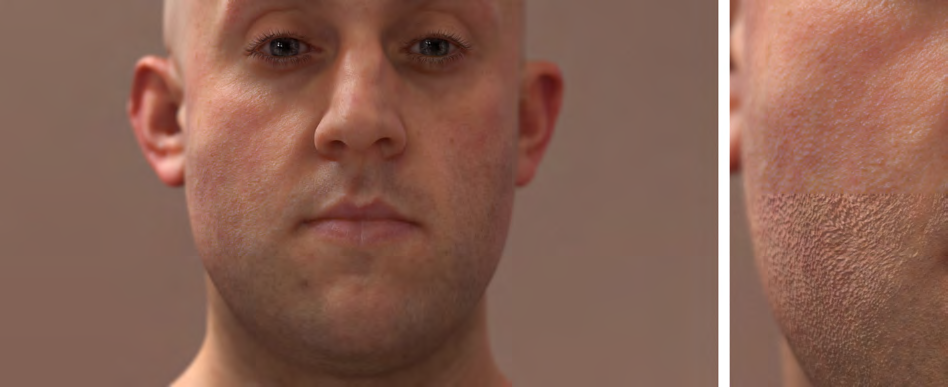
\includegraphics[width=\linewidth]{figures/sss}
    \caption[次表面散射人脸渲染效果]
    {次表面散射人脸渲染效果\citep{SpSSS}。
    在应用次表面散射之前(右下)和之后(右上)的近距离比较。}
\end{figure}
迪士尼介绍了其在离线渲染中使用的模型\citep{SSS_disney},这是对物理模型的蒙特卡洛模拟数据的数值近似。在离线渲染中,也会直接使用光线追踪对散射现象进行模拟,以达到更逼真的效果。
屏幕空间次表面散射\citep{SSSSS}在实时渲染中应用较广,其直接重用了原本渲染所需计算的数据,从而减小了开销。
纹理空间次表面散射\citep{texSSS}的提出较早,其基本思路是将会发生散射的光线先渲染在纹理空间,然后对其进行多次高斯模糊和叠加,从而计算散射效果。
\citet{SpSSS}提出牺牲一定的角对称性,以提升模糊的计算效率。
Unity3D在其渲染器中也使用了屏幕空间算法\citep{SSS_u3d},但其实现是基于\citet{SSS_disney}的模型进行随机采样,而非使用高斯模糊近似。

目前离线渲染大多使用光线追踪算法,从而直接模拟散射的过程,以确保最高的逼真度;
而实时渲染则使用屏幕空间次表面散射,以获得最高的渲染效率。
但对于多视角3D重建来说,纹理空间的方法或许更加合适,因为纹理空间的计算的结果可以被多个视角共享。

\paragraph{基于图像的光照}

除了对物理本身的建模外,对物体所处环境的准确建模也是逼真渲染的重要一环。
在早期的实时渲染中,通常使用简单的环境光照,点光源,方向光源等解析模型。
但这些模型并不能准确建模采集摄影中使用的柔光箱等设备产生的光照效果。

近年来,基于图像的光照(IBL)技术得到了广泛的应用,其基本思路是将环境光照建模为一个环境贴图,大大提升了光照建模的精度。
\citet{unreal_ssa}介绍了在Unreal Engine中所使用的分离求和近似,使环境贴图作为照明的渲染可以达到实时的效率。

\section*{本章小结}

3D人脸重建技术由于其广泛的应用前景,近年来得到了广泛的研究。
其中,使用专业设备的高精度3D人脸重建方法已经可以达到很高的精度,
其采集的速度和复杂度,所输出的模型的精度均在不断优化。
然而这类方案的成本依然十分高昂,且流程复杂,部署和调试较为困难。
对此,本文设计了一套多视角人脸数据采集方案,并在较为有限的经济和时间成本下实现了该方案,达成了较高的精度。
本文将在第\ref{chap:platform}章中详细介绍该方案的设计和实现。

此外,基于非受限环境照片的3D人脸重建方法能利用常见的照片重建人脸模型,这大大降低了人脸重建技术的应用门槛。
现有方法虽然已经能高效地重建人脸模型,但它们均未能充分利用照片中的边缘信息,导致不必要的复杂性和传递误差。
本文将在第\ref{chap:method}章中介绍如何借助可微分渲染中的可见性梯度利用这些边缘信息,
并在第\ref{chap:recon}章中介绍如何将该技术实际应用于人脸重建中。

本章还介绍了通用渲染及可微分渲染的相关技术,这些技术为本文的研究提供了基础。
